
\documentclass{article}
\usepackage{tikz}
\usetikzlibrary{arrows,shapes,trees}

\begin{document}
\section{Magic School Evolution}
\begin{center}
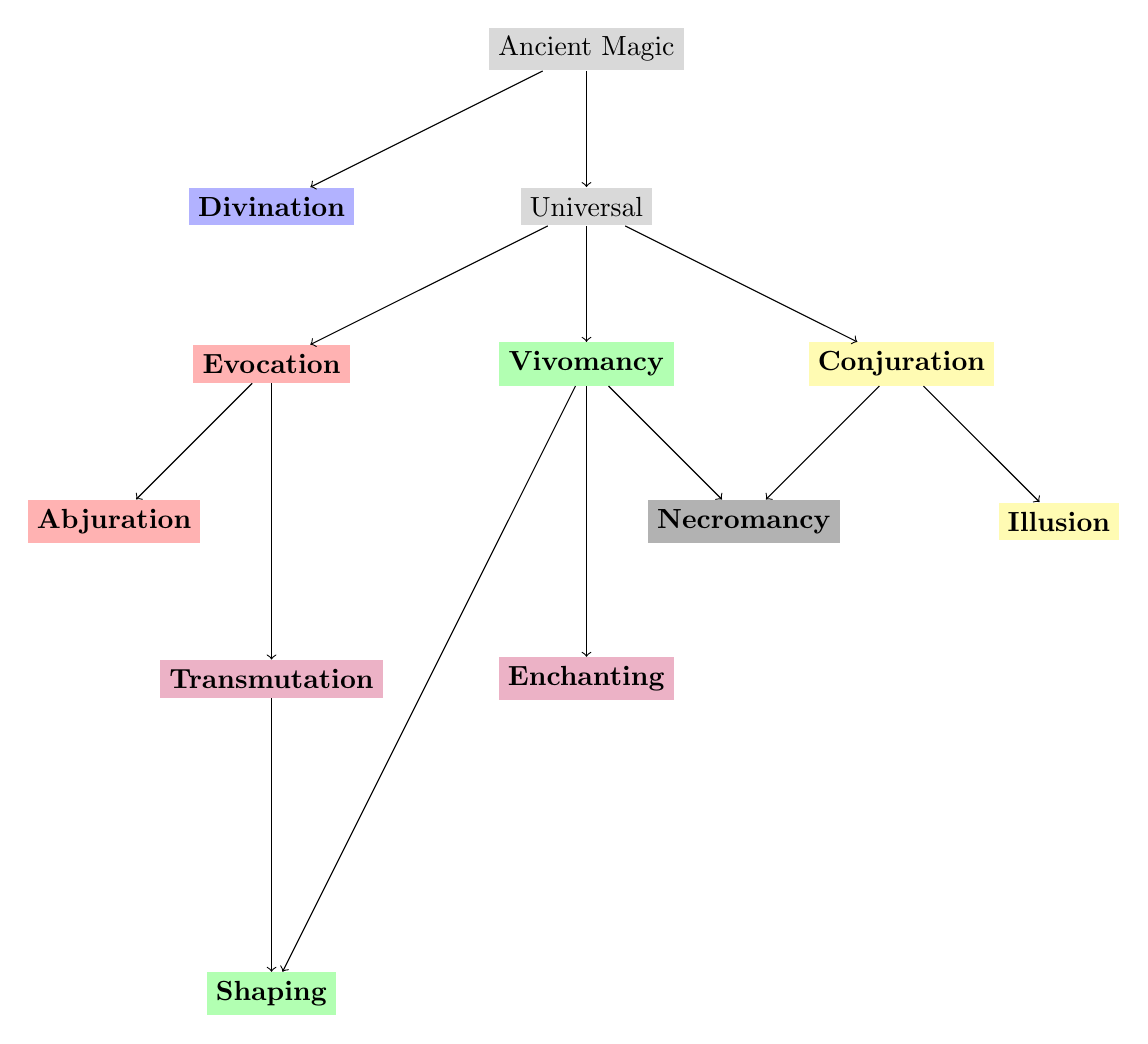
\begin{tikzpicture}[scale=2.0]
\tikzstyle{every node} = [rectangle]
\node[fill=gray!30] (root) at (3, 6) {Ancient Magic};
\node[fill=blue!30] (divination) at (1,5) {\textbf{Divination}};
\node[fill=gray!30] (univ) at (3,5) {Universal};
\node[fill=red!30] (evoc) at (1, 4) {\textbf{Evocation}};
\node[fill=green!30] (vivo) at (3, 4) {\textbf{Vivomancy}};
\node[fill=yellow!30] (conjur) at (5, 4) {\textbf{Conjuration}};
\node[fill=red!30] (abjur) at (0, 3) {\textbf{Abjuration}};
\node[fill=yellow!30] (illusion) at (6, 3) {\textbf{Illusion}};
\node[fill=black!30] (necro) at (4, 3) {\textbf{Necromancy}};
\node[fill=purple!30] (enchant) at (3, 2) {\textbf{Enchanting}};
\node[fill=purple!30] (transmute) at (1,2) {\textbf{Transmutation}};
\node[fill=green!30] (shapers) at (1,0) {\textbf{Shaping}};

\draw [->] (root) -- (divination);
\draw [->] (root) -- (univ);
\draw [->] (univ) -- (evoc);
\draw [->] (univ) -- (vivo);
\draw [->] (univ) -- (conjur);
\draw [->] (evoc) -- (abjur);
\draw [->] (conjur) -- (illusion);
\draw [->] (vivo) -- (necro);
\draw [->] (conjur) -- (necro);
\draw [->] (evoc) -- (transmute);
\draw [->] (vivo) -- (enchant);
\draw [->] (transmute) -- (shapers);
\draw [->] (vivo) -- (shapers);
\end{tikzpicture}
\end{center}

\section{Magic Schools}
\subsection{Abjuration}
Abjuration is a school focused on using magical energy for defense of the spellcaster or the target of the spell. It was an early offshoot of evocation, developed in response to evokers looking at methods of protecting themselves from their own spells. 

\subsection{Conjuration}
Conjuration is a school focused on using magic to call, summon, or create things. The earliest form of conjuration focused on calling creatures to the caster. Later forms delved into extra-dimensional summoning.

\subsection{Divination}
Divination is a school focused on the gathering of knowledge. The oldest school known, divination first appeared while humans were still in the tribal phase. Shamans and witch-doctors would cast spells to gather knowledge to help them bring their tribes to victory.

\subsection{Enchanting}
An offshoot of vivomancy, enchanting focuses on manipulation of the mind to affect the target in various ways. Enchanters are essentially the psychiatrists to the vivomancers doctors.

\subsection{Evocation}
Evocation is a school of magic focused on making things go boom.

\subsection{Illusion}
Illusion magic creates phantom images and sensations.

\subsection{Necromancy}
A perversion of vivomancy, mixed with conjuration. Necromancy focuses on manipulating corpses and life itself.

\subsection{Shaping}
A school that only existed during the Late-Cornatium era and Dominion era. Shaping draws influence from vivomancy and transmutation to create new life from existing life.

\subsection{Transmutation}
Transmutation focuses on changing the subject of the spell.

\subsection{Universal}
A catch-all, virtual school. The universal school is used to describe magic that didn't fit into any other school at the time. There has never truly been a college or group focused soley on the Universal school.

\subsection{Vivomancy}
Vivomancy is a school that uses magic to manipulate life processes of the target of their spells. Healing and wounding of the target is the most common, though there has been blending with the illusion, transmutation, and enchanting schools for various spells.

\end{document}
